
%\usepackage[spanish]{babel}
\chapter{Introducción}
El propósito de este documento es guiar al personal de pruebas a lo largo de las etapas correspondientes a la validación y/o calificación de sistemas computarizados. En el capítulo 2 se plantea el objetivo general y específicos del documento. Posteriormente en los capítulos 3,4,5 se desarrollan los protocolos estándar que permiten llevar a cabo la validación y/o calificación de un sistema computarizado, finalmente se presenta el protocolo de cierre y criterios de salida.
\chapter{Objetivos}
\section{Objetivo general}
\begin{itemize}
\item Estandarización mediante protocolo para validación y/o calificación de sistemas computarizados, tomando como elemento central la  escalabilidad, reproducibilidad y proceso efectivo de la validación y/o calificación, con énfasis en la integridad de datos.
\end{itemize}
\subsection{Objetivos especificos}
\begin{itemize}
	\item Diseñar e implementar protocolos de riesgo, validación, calificación y cierre.
	\item Demostrar si un software es adecuado para el propósito para el cual fue construido, durante todo su ciclo de vida.
	\item Comprobar el cumplimiento, con alto grado de confianza, de los requerimientos y políticas predeterminadas.
\end{itemize}
\newpage
\section{Actividades previas}
Definir e implementar, si es necesario, un ambiente dedicado de pruebas equivalente al utilizado en producción, que soporte el siguiente flujo de trabajo [Figura 2.1].
\begin{figure}[H]
	\centering
	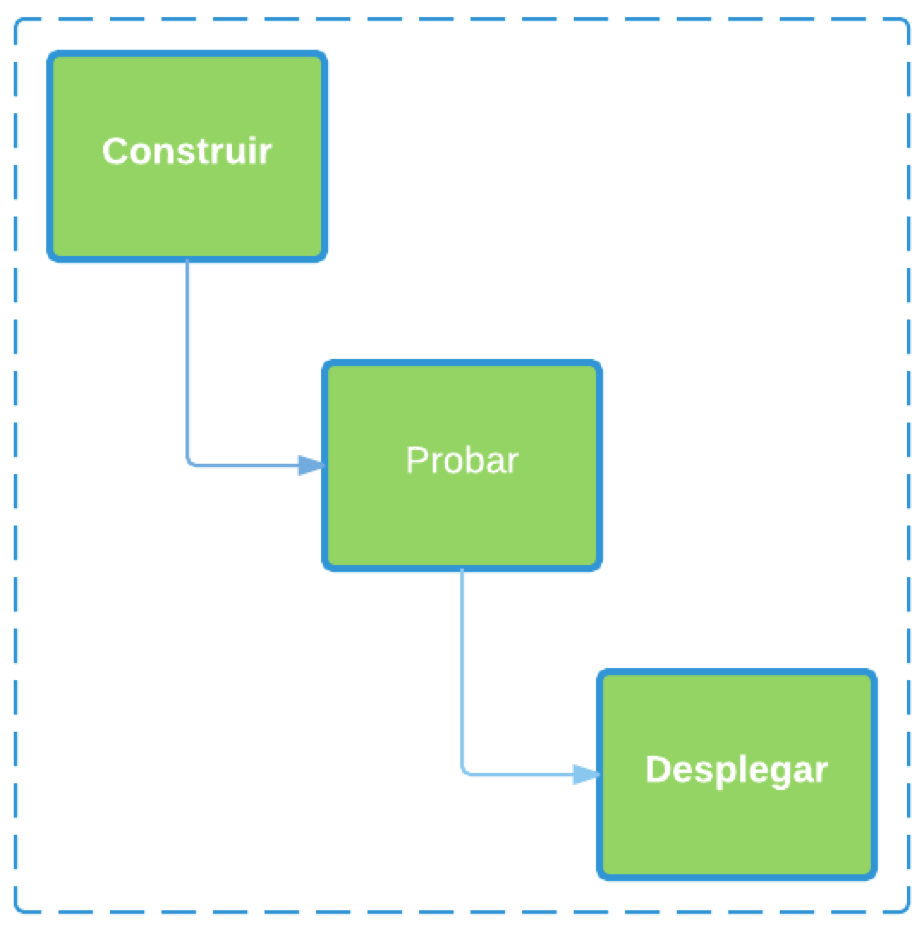
\includegraphics[width=0.3\linewidth]{img/test.png}
	\caption{Ambiente para el desarrollo de pruebas}
	\label{fig:MarcoTeorico}
\end{figure}
\section{Proceso principal}
Los procedimientos deben ser ejecutados sistemáticamente, haciendo uso de la [Figura 2.2], contexto, entendimiento de los requerimientos, documentación del desarrollo, políticas de acceso, persistencia de datos, seguridad y uso operacional del elemento a evaluar.
\begin{figure}[H]
	\centering
	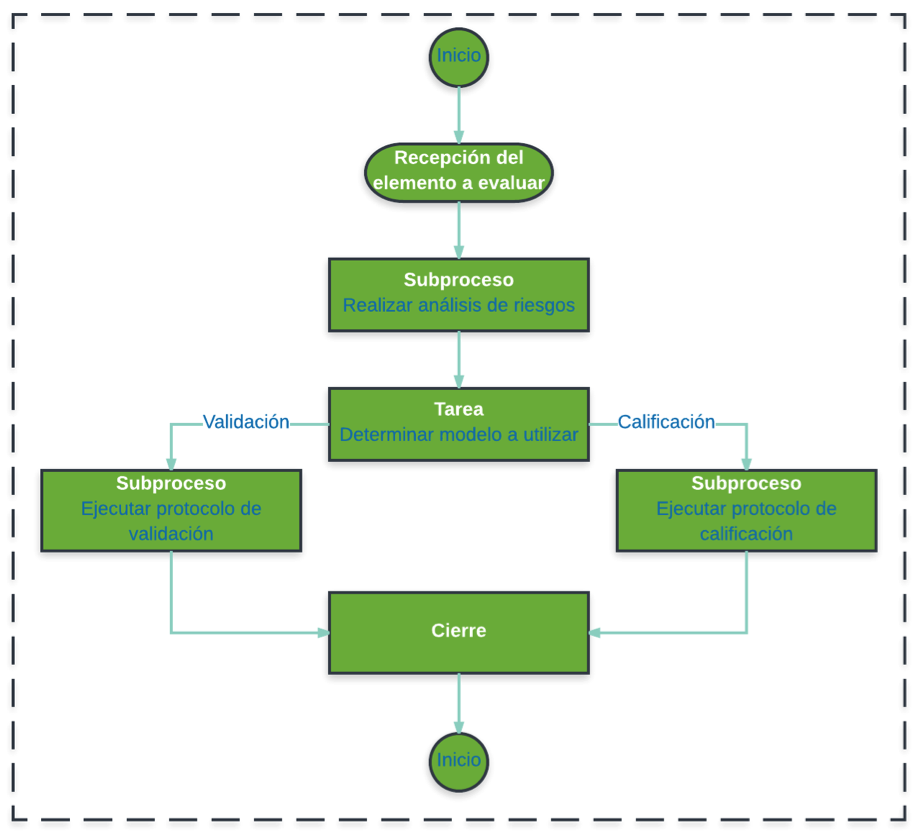
\includegraphics[width=0.5\linewidth]{img/general.png}
	\caption{Modelo general de la solución}
	\label{fig:MarcoTeorico}
\end{figure}
\chapter{Protocolo de riesgo}
El proposito de este protocolo es definir el acercamiento, metodologías, herramientas y estrategias a utilizar durante la evaluación del elemento. La administración del riesgo debe ser aplicada durante todo el ciclo de vida del software, con especial enfoque en la integridad de los datos y la calidad del estudio.
\subsubsection{Aspectos claves del diseño}
\begin{itemize}
	\item \textbf{Evaluar riesgo:} Etapa en donde se desarrollan estrategias adecuadas de validación/calificación con énfasis en la calidad e integridad de los datos. Se debe definir la metodología para llevar a cabo actividades de validación/calificación de las funcionalidades propias y asociadas al uso de sistemas computarizados.
	\item \textbf{Personal, roles y responsabilidades:} El entorno de pruebas debe contar con personal adecuado y calificado. Los roles y responsabilidades deben ser controlados y definidos  en base a un sistema de \textit{políticas de acceso}, entrenamiento y requerimientos GLP. Se debe demostrar que el personal posee los conocimientos suficientes para cumplir con el rol respectivo.
\end{itemize}
\subsubsection{Roles y responsabilidades}
A este nivel de la evaluación se debe corroborar si los roles y responsabilidades son desarrollados conforme a los principios y estándares GLP. Es preciso especificar el entrenamiento, competencias y habilidades del personal relevante dentro del ciclo de vida del software.
\begin{enumerate}	
	\item Director QA.
	\item Personal QA.
	\item Usuarios de operación.
	\item Expertos de validación.
	\item Personal de soporte y mantención.
	\item Proveedores.	
\end{enumerate}
\subsubsection{Control del cambio y configuración}
\begin{itemize}	
\item Los cambios realizados a los sistemas computarizados deben ser de acuerdo a los procedimientos para control del cambio.
\item Deben estar definidos los roles y responsabilidades asociadas a las actividades del control de cambios.
\end{itemize}
\newpage
\subsubsection{Entradas del proceso}
\begin{enumerate}
\item Nombre, versión y descripción clara del propósito del elemento a evaluar.
\item El hardware en donde opera el elemento.
\item El sistema operativo y otras herramientas que trabajen en conjunción con el sistema computarizado.
\item Lenguaje de programación y/o sistema de almacenamiento de datos.
\item Principales funciones del sistema evaluado.
\item Descripción de los flujos y tipos de datos.
\item Manejo de excepciones.
\item Describir la comunicación e integración con otros módulos o sistemas.
\item Describir procedimientos para la detección y prevención de accesos no autorizados.
\item Describir procedimiento de mantención y reparación.
\item Procedimientos para el desarrollo de software, pruebas de aceptación y otras pruebas relevantes.
\end{enumerate}
\subsubsection{Las actividades correspondientes a este nivel son}
\begin{itemize}
\item Determinar el acercamiento de la evaluación.
\item Definir el flujo de trabajo, tareas y roles del equipo de trabajo.
\end{itemize}
\subsubsection{Salida}
\begin{itemize}
	\item Estrategia de validación y/o calificación.
\end{itemize}
\chapter{Protocolo de validación}
Este proceso consiste en una serie de actividades que son ejecutadas individualmente. El propósito de la validación es proveer información que asegure la calidad de un sistema computarizado.
\subsubsection{Los procesos deben ser realizados en estricto orden secuencial}
\begin{enumerate}
	\item Plan de pruebas y control.
	\item Análisis y diseño de pruebas.
	\item Ejecución de las pruebas
	\item Evaluación del criterio de salida y reporte.
\end{enumerate}
\section{Plan de pruebas y control}
El propósito de esta etapa es definir la misión de las pruebas, objetivos y decisiones necesarias para transformar la estrategia de validación en un plan operacional, las entradas en que se basa este proceso son:
\begin{itemize}
	\item Estrategia de validación.
	\item Plantilla plan maestro de pruebas.
	\item Información sobre el progreso de las pruebas.
\end{itemize}
\subsubsection{Las actividades correspondientes a este nivel son:}
\begin{itemize}
\item Veririficar la estrategia y definir el objetivo de las pruebas.
\item Ejecutar acciones correctivas al plan maestro de pruebas.
\end{itemize}
\subsubsection{Salida}
\begin{itemize}
\item Plan maestro de pruebas.
\end{itemize}
\section{Análisis y diseño de pruebas}
El propósito de esta etapa es producir el diseño pruebas, junto con sus condiciones, casos y datos de prueba, acorde al nivel genérico de pruebas de software [Figura 4.1].
\begin{figure}[H]
	\centering
	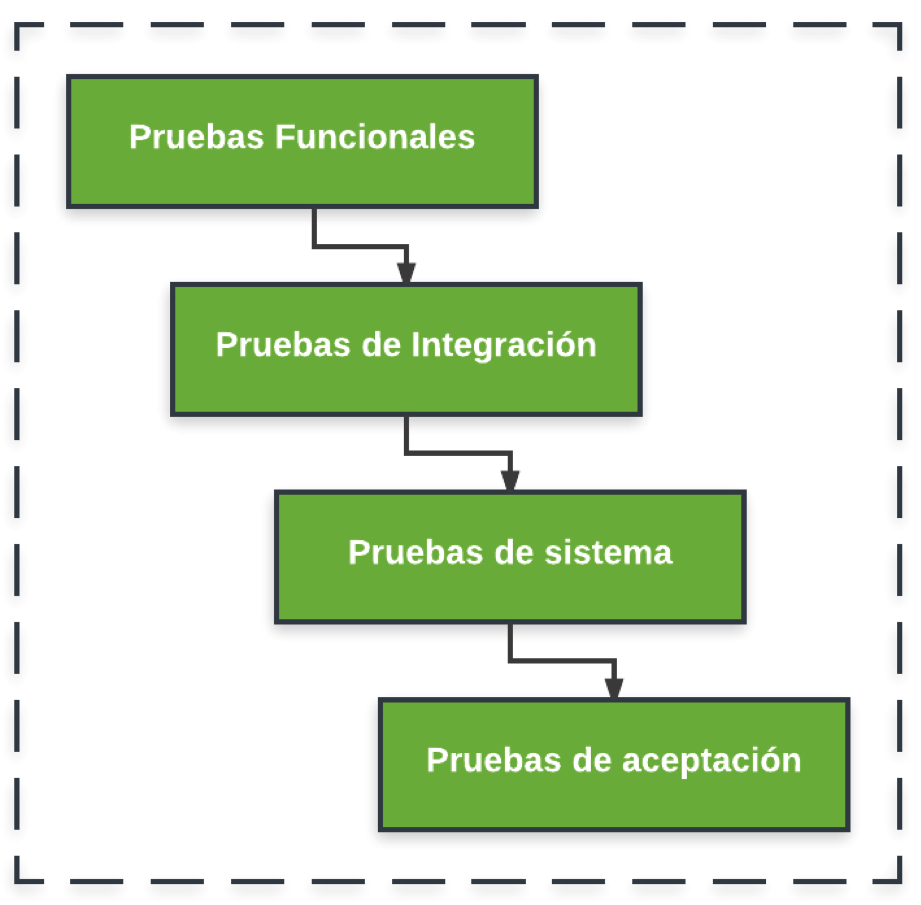
\includegraphics[width=0.5\linewidth]{img/pruebas.png}
	\caption{Nivel genérico de pruebas}
	\label{fig:MarcoTeorico}
\end{figure}
\newpage
\subsubsection{Entradas de este proceso:}

\begin{itemize}
	\item Plan maestro de pruebas.
	\item Nivel genérico de pruebas.
	\item Manual de usuario.
\end{itemize}

\subsubsection{Las actividades correspondientes a este nivel son:}

\begin{itemize}
	\item Análisis de la documentación recopilada.
	\item Especificación de los niveles de prueba acordes a la estrategia validación.
\end{itemize}

\subsubsection{Salida:}
\begin{itemize}
	\item Nivel especifico de pruebas.	
\end{itemize}

\subsection{Diseño de las pruebas}

\subsubsection{Pruebas funcionales}

Las pruebas son del tipo caja negra [Figura 4.2]. Se examinan y registran en la [Tabla 4.1] las salidas del sistema, sin importar el funcionamiento interno del módulo inspeccionado, la respuesta de la ejecución es medida según criterio establecido en la \textit{métrica de resultados}, presentada en la [Tabla 4.2].

\begin{figure}[H]
	\centering
	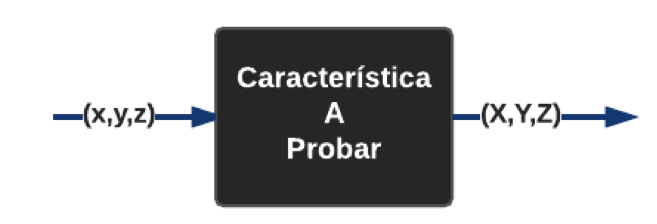
\includegraphics[width=0.6\linewidth]{img/cajanegra.png}
	\caption{Diagrama de entrada y salida}
	\label{fig:MarcoTeorico}
\end{figure}

\begin{table}[htbp]
	\begin{center}
		\begin{tabular}{|l|l|}
			\hline
			Función a probar & Caso de prueba \\
			\hline \hline
			Entrada valida		 &  \\ \hline
			Salida esperada &  \\ \hline
			Entrada invalida &  \\ \hline
			Salida esperada & \\ \hline
			\hline \hline
			Resultado: & \\ \hline
			
		\end{tabular}
		\caption{Plantilla genérica de ejecución}
		\label{tabla:sencilla}
	\end{center}
\end{table}

\newpage

\subsubsection{Métrica de resultado}

\begin{table}[H]
	\begin{center}
		\begin{tabular}{| p{3cm} | p{7cm} | p{1cm} |}
			\hline
			Resultado & Definición & Sigla \\
			\hline \hline
			Error Humano & Acción Humana que produce un resultado incorrecto & M \\ \hline
			Defecto & Paso, proceso o definición de datos incorrecto & D \\ \hline
			Falla &la incapacidad de un componente para realizar la función requerida
			dentro de los requisitos de funcionamiento especificados.  & F \\ \hline
			Error & Diferencia entre el valor medido y el teórico & E \\ \hline
			No aplica & Sin hallazgos & n/a \\ \hline
		\end{tabular}
		\caption{Métrica de evaluación}
		\label{tabla:sencilla}
	\end{center}
\end{table}

\section{Ejecución de las pruebas}

El propósito de esta etapa es organizar los casos de prueba en procedimientos, para luego ejecutar las pruebas físicas en el ambiente correcto.

\subsubsection{Entradas de este proceso:}

\begin{itemize}
	\item Nivel especifico de pruebas.
	\item Condiciones y diseño de pruebas.
	\item Plantilla de ejecución.
\end{itemize}

\subsubsection{Las actividades correspondientes a este nivel son:}
\begin{itemize}
	\item Organizar procedimientos.
	\item Verificar el ambiente de pruebas.
	\item Ajustar la plantilla de ejecución.
	\item Ejecutar las pruebas.
	\item Registrar las pruebas.
	\item Analizar y medir los resultados.
\end{itemize}

\subsubsection{Salida:}

\begin{itemize}
	\item Registro de las pruebas.
	\item Reporte de incidentes.
\end{itemize}

\chapter{Protocolo general de calificación}

La calificación formal es aceptable cuando el elemento a evaluar es un producto de caja (COTS), equipo automatizado o software sencillo.  

\subsubsection{Entradas de este proceso:}

\begin{itemize}
	\item Manual de usuario.
\end{itemize}


\subsubsection{Las actividades correspondientes a la calificación son:}

\begin{itemize}
	
\item Configuración: Primero el elemento a calificar debe ser instalado/configurado en conformidad con los requisitos recomendados por el fabricante o desarrollador.

\item Calibración: Los mediciones y valores obtenidos por equipos automatizados deben ser comparados con los obtenidos por un instrumento de medición calibrado.

\item Pruebas funcionales: Este nivel de prueba se basa en el principio de caja negra, la inspección de las funciones se realiza mediante la alimentación de entradas y posterior evaluación de las salidas. Cada prueba es aislada en un escenario de uso con sus correspondientes casos de prueba [Figura 5.1].

\begin{figure}[H]
	\centering
	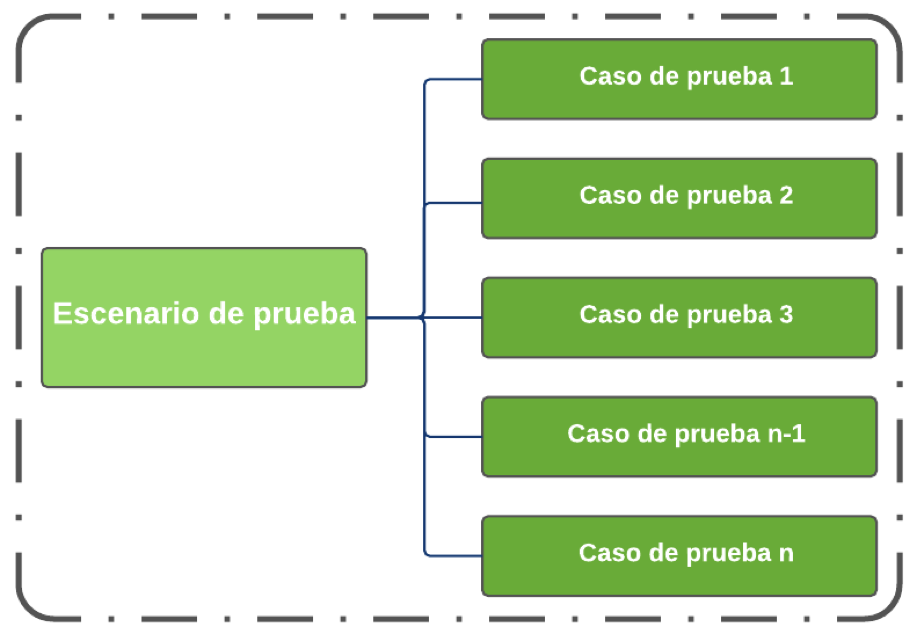
\includegraphics[width=0.5\linewidth]{img/funcional.png}
	\caption{Modelo prueba funcional}
	\label{fig:MarcoTeorico}
\end{figure}

\end{itemize}

\subsubsection{Salida:}

\begin{itemize}
	\item Registro de las pruebas funcionales.
	\item Reporte de incidentes.
\end{itemize}

\chapter{Evaluación del criterio de salida y reporte}

El propósito de esta etapa es documentar y entregar resultados finales, en un formato entendible a los stakeholders.

\subsubsection{Entradas de este proceso:}
\begin{itemize}
	\item Estado de avance.
	\item Documentación y resultados de la ejecución de las pruebas.
\end{itemize}

\subsubsection{Las actividades correspondientes a este nivel son:}

\begin{itemize}
	\item Comparar los resultados obtenidos con lo esperado/planeado.	
	\item Documentar resultados de las pruebas.
\end{itemize}

\subsubsection{Salida:}
\begin{itemize}
	\item Presentación final correspondiente a la validación y/o calificación.
	\item Reporte IQ, DQ, OQ, PQ.
\end{itemize}
